\documentclass[11pt]{article}
    \title{\textbf{NCSU ECE492/592 Mothership Final Report}}
    \author{Robby Rivenbark, Alex Pendergast, Daniel Smith, Jake Carter, and Dallin Yost}
    \date{Spring 2022}
    \usepackage[margin=0.75in]{geometry}
    
\usepackage{graphicx}
\usepackage[numbers]{natbib}
\begin{document}
\maketitle

\section{Abstract}

The goal of this project was to design an Unmanned Aircraft System (UAS) that would launch a SAM4 drone (the Mothership) with a small 5-inch racing quad (the Babyship) attached to its underside. Teams from other undergraduate programs have attempted a project similar to this in the past, but did not make very much progress. Our team had a unique set of skills that we felt would improve upon the previous teams' attempts. For our attempt at this project, the Mothership would fly to a predetermined altitude and release the Babyship. The Babyship would detect when it has been released and catch itself midair. Once the Babyship catches itself and stabilizes, it will fly to a location, determined at launch time, and land. During this time the Mothership will loiter while waiting for a “landed” signal from the Babyship to come pick it up. At which time the Mothership would approach the Babyship’s location, descend to where it can visually identify the Babyship and begin its final approach. The Mothership will track the visualizer on the Babyship to guide a carbon fiber rod into a cage on top of the Babyship. Once the Mothership has received confirmation that the Babyship has been caught on the retrieval mechanism via a limit switch, the rod will move into a holding position to secure it and then return to launch. We were able to successfully complete each of these objectives individually, but found integration to be somewhat difficult.
\section{Introduction}

This project involves the design and fabrication of an unmanned aerial system composed of two drones - a Mothership and a babyship. The Mothership’s role in the system is to transport, release, and retrieve the babyship. It is fitted with a payload designed to perform these roles. For our project, the babyship had no payload of its own - it was only fitted with communication and positioning equipment, along with a pickup structure to assist with release and retrieval.\\\\
\noindent
This type of UAS has applications in search and rescue, reconnaissance, and defense. If someone goes missing in an environment with dense tree cover, traditional aerial search and rescue methods may be inefficient. A Mothership could transport a host of smaller UAVs into the search area to be deployed into areas that larger drones or vehicles may be unable to reach. Similarly, if the babyships were fitted with weaponry or observation equipment, the same benefit of reaching spaces that are harder for larger vehicles to maneuver around could be extended to defense or reconnaissance.\\\\
\textbf{Our contributions are as follows:}
\begin{description}
    \addtolength{\itemindent}{1.0cm} 
    \item[Robby Rivenbark] Image recognition programming, mission programming
    \item[Alex Pendergast] Mission programming, babyship assembly and testing
    \item[Dallin Yost] Payload design and fabrication
    \item[Jake Carter] Payload design and fabrication
    \item[Daniel Smith] Babyship assembly and testing
\end{description} 
\section{Related Work}

The United States Department of Defense has made significant progress testing an “aircraft carrier in the sky” capable of transporting multiple smaller UAVs into a theater of operations while maintaining a constant air presence. Their research primarily focuses on safe release of fixed-wing UAVs from manned military aircraft such as the C-130, F/A 18, and P-8A. The release mechanisms of these drones are adapted from existing aircraft payload systems: Boeing is partnering with the DoD to research a canister-based system to carry and launch drones mid-flight on the weaponry systems of fighter jets, and BAE Systems is developing a system to deploy drones from the P-8A maritime patrol aircraft’s sonobuoy launch systems. These applications involve defense and reconnaissance - for example, the P-8A child UAVs would have magnetic anomaly detection equipment to assist in the detection of submarines.\cite{garrun_2015}\\\\
Researchers in Belgium conducted an experiment involving the mid-flight release of a child UAV from a mother UAV. Their experiment is close in scale to our own, as they launched a Parrot AR Drone 2.0 off of a DJI Phantom 2. These researchers designed a 3D-printed release payload for the mother UAV and a corresponding mechanism on the child UAV. They found that the DJI Phantom 2 could not carry the weight of the payload and the child UAV on its own, so the child had to assist in vertical thrust. They also discovered that turbulence from the mother UAV’s propellers would disrupt the release stabilization, so they developed a winch system on the release payload to control the release distance. Their experiment also detailed the control design used to stabilize the child UAV using a PID controller. Finally, their experiment did not include any retrieval programming or mechanisms.\cite{inproceedings}\\\\
In a senior capstone project and later a conference paper from the University of Florida Tech Aerospace Engineering department a team of engineers were working towards mid air docking between a fixed wing aircraft and a quadcopter. The team has a multirotor drone separate mid flight to complete an autonomous delivery and then autonomously return to the fixed wing aircraft flying at a constant speed to dock. Location of the fixed wing aircraft is through on board image recognition of a black and white pattern using OpenCV. Initial testing demonstrated the feasibility of the team's docking assembly and the ability to re-dock at fixed wing aircraft speed in a manual human operated test flight.\cite{9438229}\\\\
In a project from the University of California Berkeley's High Performance Robotics Laboratory a team has implemented a flying system for recharging a drone mid-flight through two smaller drones that land on top of the main drone. This design is a prime example of mid flight autonomous landing of one drone on another drone.  The battery drones landing to recharge the main drone successfully demonstrates a dual quadcopter Mothership configuration as well as a potential use. This project was successful in running autonomous code to land drones together mid flight; it does so in a completely controlled indoor environment.\cite{9197580}\\
\section{Approach}

We constructed the miniature drone entirely from scratch as a part of the project. The “Babyship” is a 5”-propeller racing quadcopter. It is controlled through an RFD 900X SiK radio used for telemetry and for RC control. The baby ship features a canopy constructed from wire and construction paper that serves as the mechanism for dropoff and pickup. The full list of parts used to construct the Babyship can be found in Appendix C.\\\\
\begin{figure}[htp]
    \centering
    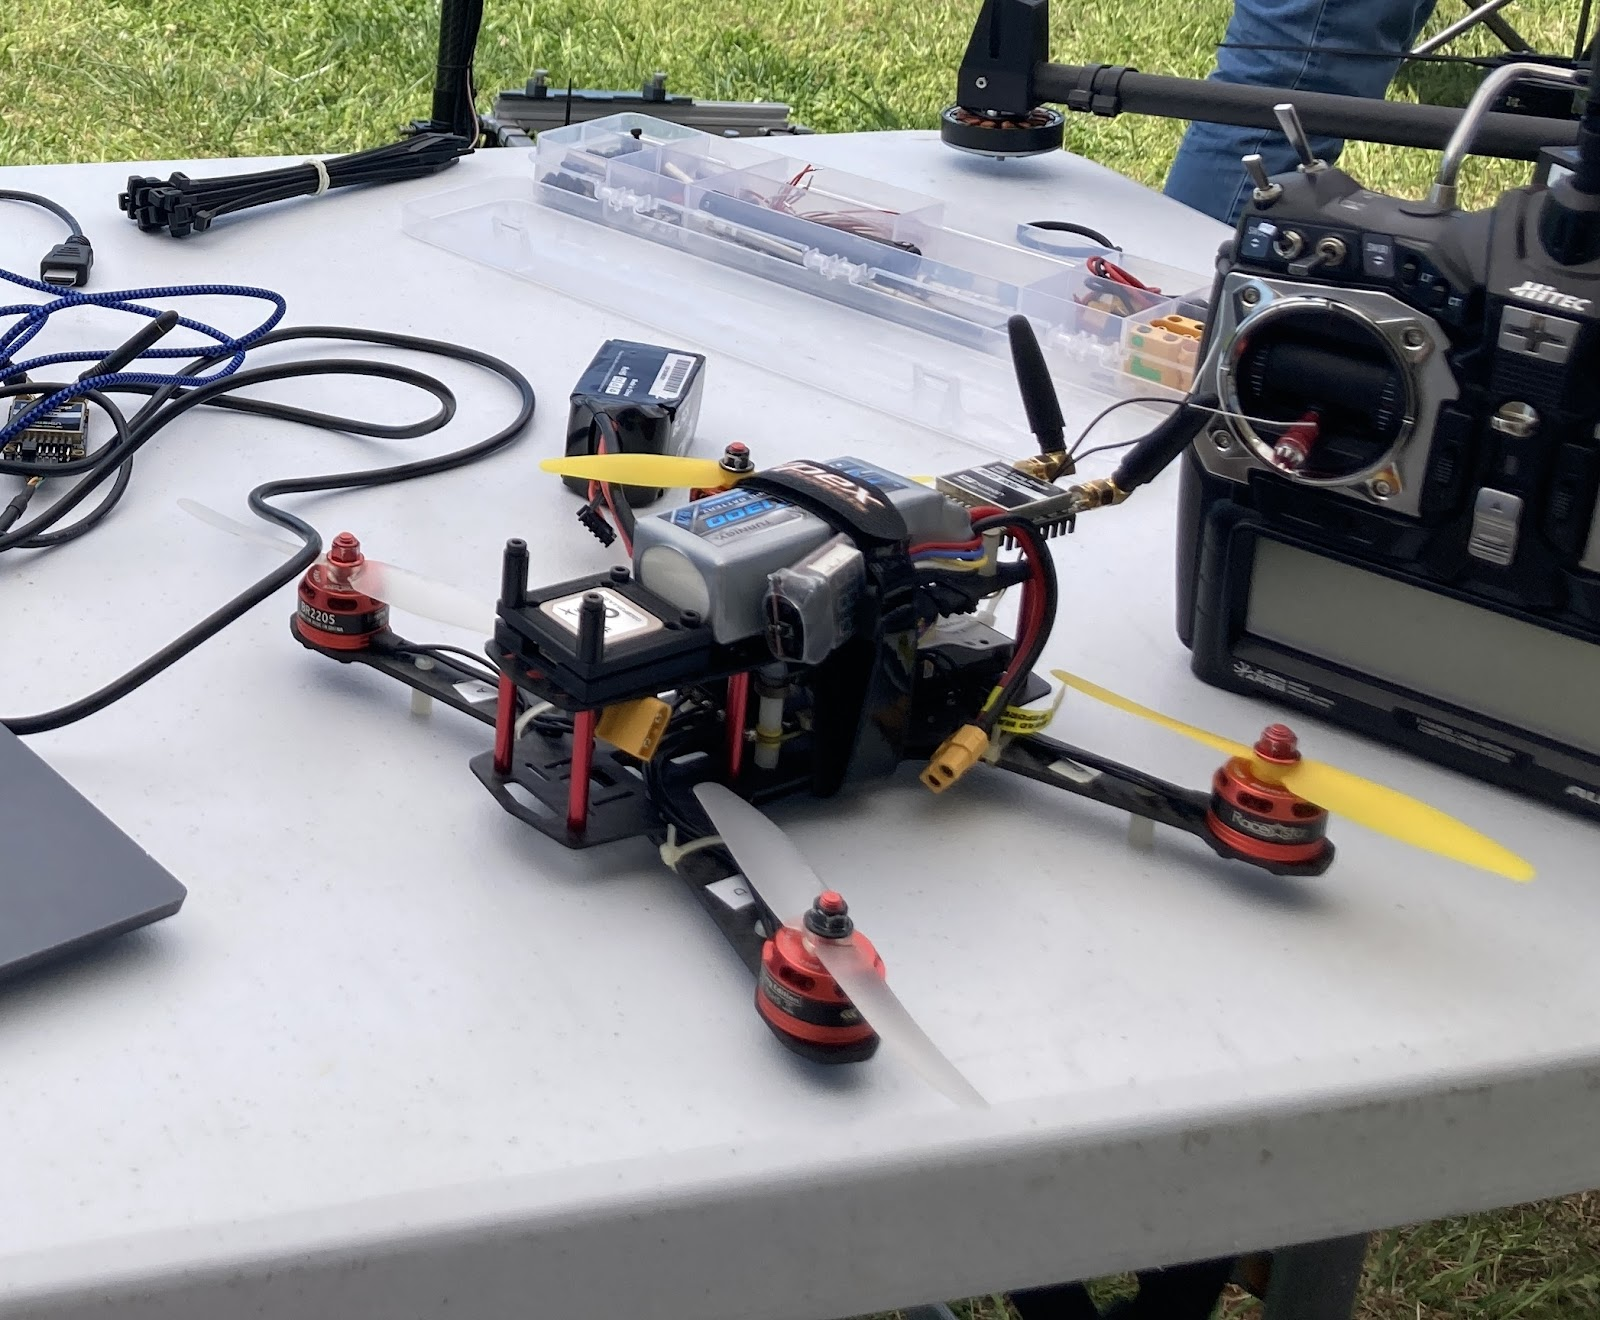
\includegraphics[scale=0.15]{Babyship.png}
    \caption{Babyship without catch/release canopy attached}
\end{figure}\\
\noindent
To complete the task two autonomous drones had to be flown at the same time. To accomplish this additional hardware was added to the payload attached to the Mothership, an interchangeable SAM4 drone. Most importantly is the addition of a raspberry pi to the payload allowing the Mothership to process images and control servos on the drone. A full list can be found in Apendix D The diagram describing connections between hardware and communication between the drones and ground control computer are outlined in Figure 2.
\begin{figure}[htp]
    \centering
    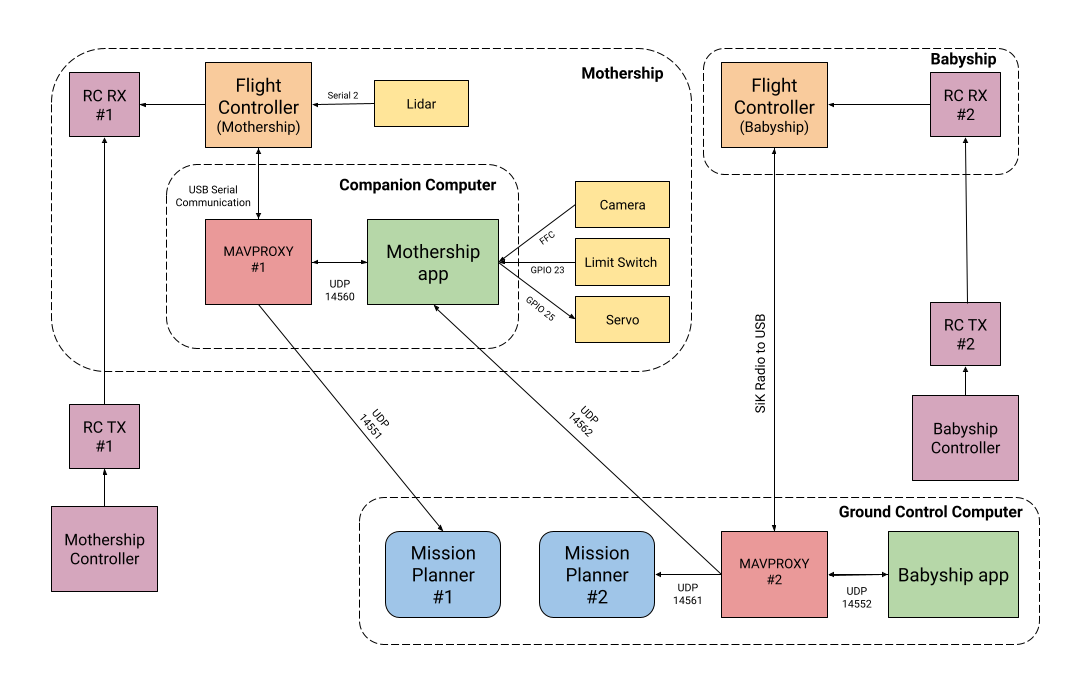
\includegraphics[scale=0.3]{Communication_Diagram.png}
    \caption{Communication Diagram}
\end{figure}
\subsection{Payload}
For the sake of the modularity of the Mothership, an interchangeable payload designed to connect to the underside of a SAM4 drone was constructed. This payload was designed to house our Raspberry Pi companion computer, the additional sensors not included on the SAM4 that the Mothership would need to accomplish its purpose, and the mechanism to pick up, carry, and drop the Babyship. The frame of our payload was constructed from two CNC cut, carbon fiber mounting plates connected by four standoffs. In order to mount a servo, limit switch, camera, and LiDAR sensor, along with the Babyship carrying mechanism to the payload, five mounting structures were 3D printed. The Babyship carrying mechanism consists of a 3D printed pivot point, two 3D printed clamps, a carbon fiber rod, and a servo. The servo allows the carbon fiber rod to pitch up and down, either securing the Babyship for carrying, or releasing the Babyship. The entire payload assembly was created using the Onshape CAD software.
\begin{figure}[h]
    \centering
    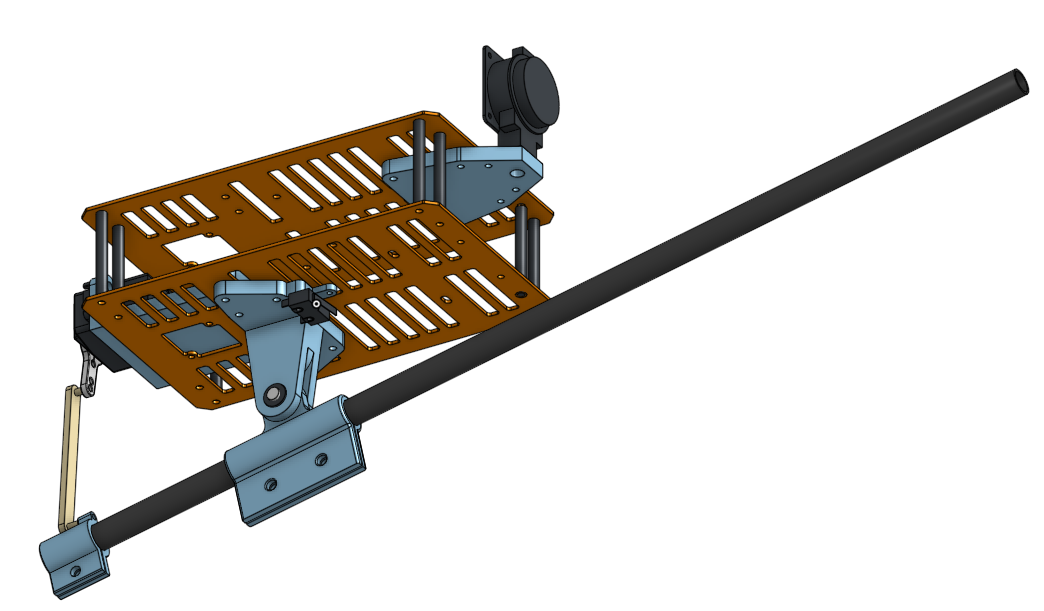
\includegraphics[scale=0.3]{Payload_Assembly.png}
    \caption{Payload Assembly in CAD}
\end{figure}
\begin{figure}[htp]
    \centering
    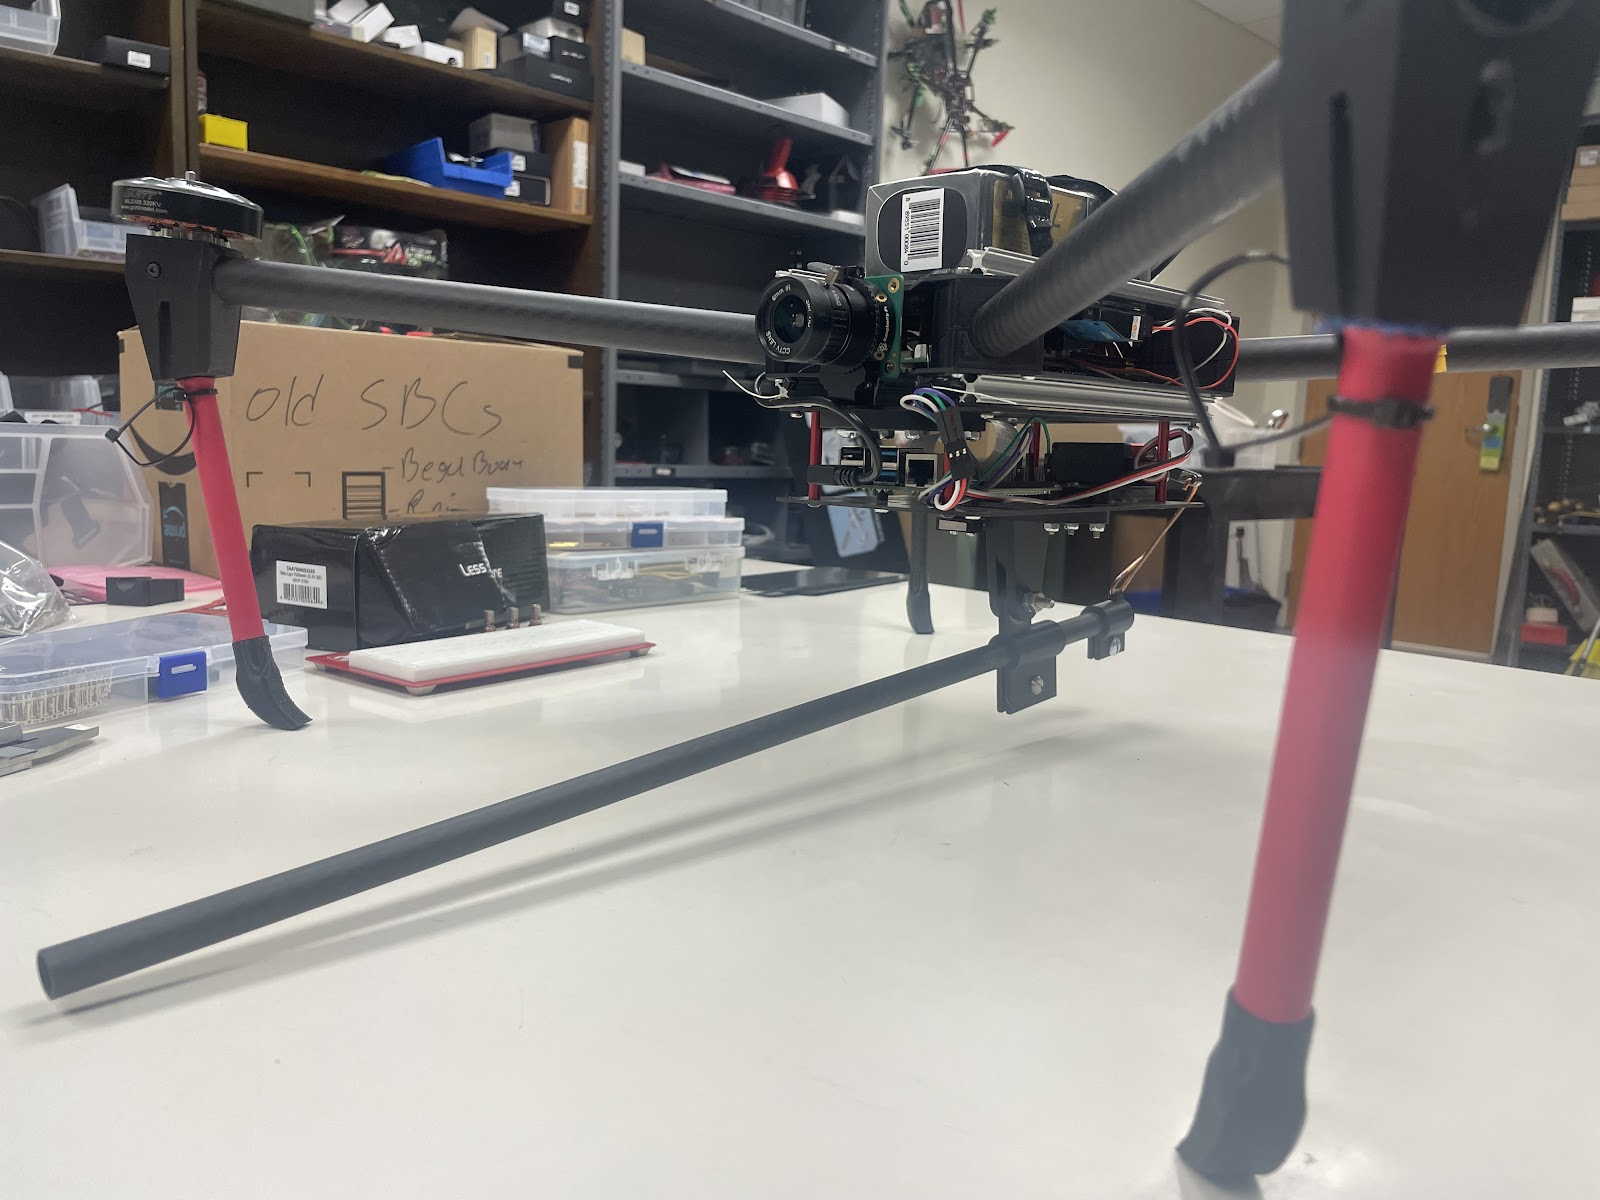
\includegraphics[scale=0.2]{Payload_Constructed.png}
    \caption{Payload constructed and mounted on SAM4}
\end{figure}
\subsection{Visualizer and Retrieval Cage}
In order to retrieve the Babyship the Mothership needed something to track as well as something to grab onto. Because of space and size constraints, it was ideal to find a way to combine the two components into one.  Our first design was a red ring on a pole sticking up from the top of the Babyship (see figure 5 below), but after careful consideration, we determined that we would need a better design that would be easier to see and catch.\\
\begin{figure}[htp]
    \centering
    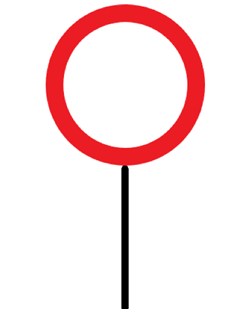
\includegraphics[scale=0.3]{Visualizer_Cage.png}
    \caption{One of the earliest Retrieval Component and Visualizer designs}
\end{figure}\\
We also considered using an electromagnet on the Mothership and a permanent magnet on the Babyship for catch and release. However, after testing the compass calibration with small magnets nearby, we determined that the magnets required to lift and hold the Babyship would interfere with the compass on both drones making it almost impossible to fly them. Our final retrieval component design looks something like a minimalistic bird cage with only 4 of the supports in an interlocking arch formation and can be seen in Figure 6. This allowed for more space for the grabber arm to penetrate, and enough area to design a visualizer for the Mothership to lock on to. Until recently, our visualizer design was a 4-inch diameter Styrofoam ball that would sit on top of the cage as seen in Figure 6 and Figure 7
\begin{figure}[htp]
    \centering
    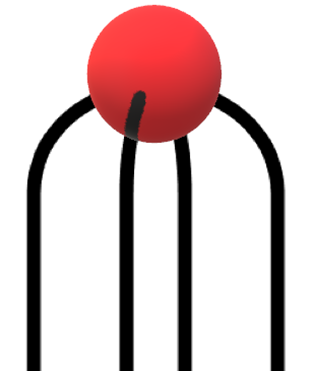
\includegraphics[scale=0.3]{Ball.png}
    \caption{Final Retrieval Component design with red ball on top}
\end{figure}\\
\begin{figure}[htp]
    \centering
    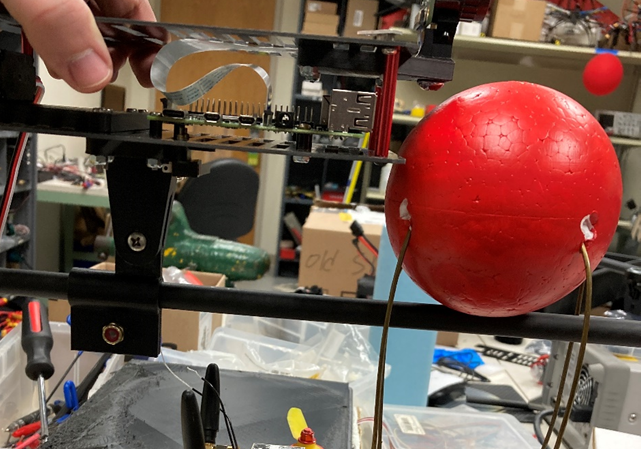
\includegraphics[scale=0.3]{Ball_Constructed.png}
    \caption{The Red Ball was unable to fit under the payload sled}
\end{figure}\\
To compound this problem, our tracking code had a hard time tracking the round, reflective surface. Considering these issues, we eventually switched to a flat, matte sheet of brightly colored paper. Doing so was a pretty simple switch; we removed the ball and draped a sheet of paper over the cage and attached it only on the top side leaving the sides to flap freely. This design gave us greater ability to track the Baby ship due to the larger, more consistently colored surface, as well as catch the drone within the limited space under the Mothership. The final design can be seen below in Figure 8. 
\begin{figure}[htp]
    \centering
    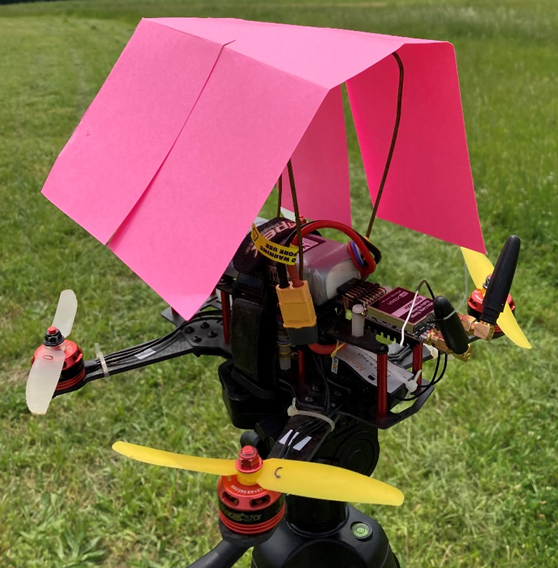
\includegraphics[scale=0.3]{Babyship_Canopy.png}
    \caption{Final visualizer and retrieval cage design}
\end{figure}\\
During the design phase of this project there were other ideas for solving the issues we dealt with above that we may have explored given more time and means. Having more space under the Mothership would have given us room to create a better visualizer. This could be done by using longer legs on the Mothership. However, this leads to needing a larger cage on the Babyship which adds mass, as well as increasing the odds of destabilizing the Babyship in flight. We saw this while adjusting the size of the visualizer from a large sheet to a smaller one. Another proposed solution was to create a landing pad for the Mothership with a slit going down the center of it so that the Babyship could hang underneath without hitting the ground. However, a lot of these issues would be mitigated by doing the retrieval with both drones in the air. This was ultimately our final goal, but to make testing our UAS simpler, we wanted to start by catching the drone on the ground and once that was achieved, try to catch it in the air.
\subsection{Image Processing and Precision Control}
At a high level image processing allowed the Mothership to seek the Baby out given that the Mother was between 2.5 and 3.5 meters south of the Baby, center vertically on the Baby, center horizontally on the Baby, and advance towards the Baby for retrieval.\\\\
\noindent
OpenCV was used to recognize the visual indicator on the Babyship. This was done by taking the output of the camera, doing a gaussian blur on the image, and then creating multiple black-and-white masks using the blurred image and carefully tuned hsv filters. Then all of these masks were combined together using a logical “or”, some basic processing was done to remove noise and fill in gaps, and the largest contour was taken to be the visual indicator. The normalized position of this contour in the frame was then used to calculate commanded forward, horizontal, and/or angular (yaw) velocities for the Mother to be moved by.
\section{Experimental Results and Analysis}
While our final submission was not able to complete the whole intended flow of the project at once, we had many successful results from individually running smaller parts of the whole task.
\subsection{Pickup Routine}
Testing in SITL as well as in the field the ability for the Mothership and Babyship to wirelessly communicate and for the Mothership to locate, fly to, and land within 3 meters of the Babyship.
Figure 9 show detection using our finalized thresholds.These ended up being quite robust: able to consistently detect the target in various light conditions and at various angles relative to the sun.
Figure 10 shows the Mothership correctly centered on the baby after flying to its GPS coordinates. This indicates the correct functionality of the seeking algorithm, the vertical centering algorithm and the horizontal centering algorithm.
\begin{figure}[htp]
    \centering
    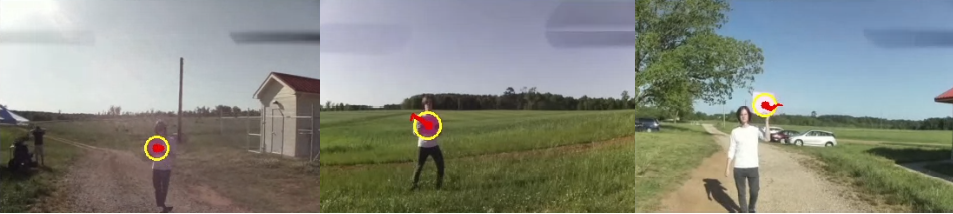
\includegraphics[scale=0.6]{All_Directions.png}
    \caption{Successful detection facing Northwest, North, and East}
\end{figure}
\begin{figure}[htp]
    \centering
    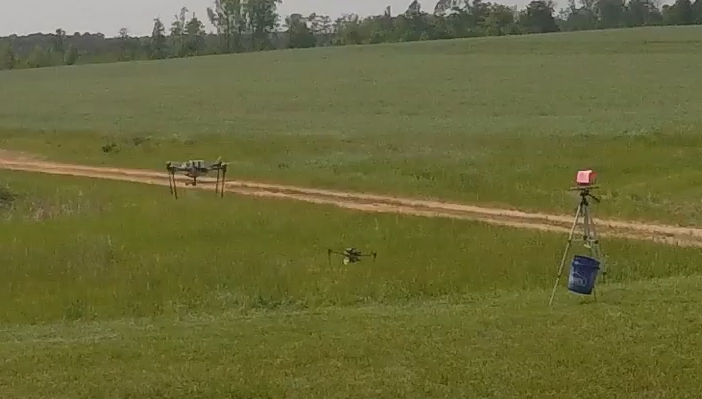
\includegraphics[scale=0.5]{Centering.png}
    \caption{Successful vertical and horizontal centering}
\end{figure}\\
Two main factors prevented the pickup routine from working entirely:
\begin{enumerate}
    \item Although the initial vertical and horizontal alignment worked, the mother would quickly lose altitude as it advanced.
    \item There was no protocol implemented to read input from the limit switch and determine that the baby was correctly picked up.
\end{enumerate}
These problems are absolutely possible to solve given time. The loss of altitude could likely be solved by either continuing to issue vertical velocity commands to the mother as it advances  or by using the lidar sensor to maintain the altitude that the mother is at when vertically centered. The  limit switch issue could be solved by running a separate thread that polls the value of the limit switch and as soon as it goes off, the vision loop is exited.
\subsection{Drop Off Routine}
The primary area of concern for the dropoff routine was the question of whether or not throw mode would work to allow the baby to stabilize itself in the air after being dropped. To answer this question the Mothership was flown, carrying the Babyship,  to a height of 10 meters. From there the grabber arm was set to release and the Babyship plummeted about 5 meters before abruptly catching itself in a stable hover. This is consistent with Ardupilot’s documentation of throw mode, which states that 10 meters is the recommended drop distance.\\\\
These results clearly show that the use of throw mode would allow for a viable midair release of the Babyship from the Mothership. The main issue that currently prevents the dropoff routine from working entirely is that the baby’s home position is set when it is armed, which is high up in the air. This causes the baby to land very slowly because it expects the ground to be 10 meters higher than where it is.
\subsection{Flying Rough}
For the additional objective “flying rough with the baby” the Mothership was flown by a safety pilot, with the Babyship attached, in loiter mode for a full minute of simulated rough flight. The Babyship did drop during a lunge forward at speed. Video analysis shows the point of failure to be the arm shifting from the hold position to the release position. The cause of this failure is unknown at this point, it is possible that the wire slipped out of the servo arm, a screw came loose, the code failed, or overpowering the servo. Further testing is needed to test this mechanism in different conditions to ensure this aspect of the payload is functioning. No problems arose for the grabber arm during our full demonstration which involved a full takeoff, flight, and drop of the Babyship. For short slow flights the current implementation should be sufficient.


\section{Conclusion}
The Mothership project came close to achieving its stated goal, with many crucial subsystems working properly, but due to technical problems and time constraints fell short of a fully integrated pickup and dropoff routine. Successes for the project includes a fully functional “baby” racing drone, a usable visual indicator on the Babyship, a working payload on the Mothership with a servo-driven arm, functional mission code for the Mothership to land approximately 3 meters south of the Babyship, and functional seeking, horizontal centering and vertical centering algorithms using computer vision and velocity control.\\\\
The main areas of focus for a future team to take this over would be better vertical stabilization of the mother when advancing, using the output of the limit switch to determine if the baby has been successfully retrieved, and dealing with the discrepancy of the baby’s home position and the mother’s home position. These problems are solvable using the design that our team implemented and this project could be completed within another semester given another dedicated and technically proficient team.

\bibliographystyle{IEEEtranN}
\bibliography{FinalReport}

\section*{Appendix}
\subsection*{Appendix A: Paramters changed to enable dropping the Babyship}
THROW\_TYPE = 1\\
THROW\_MOT\_START = 0\\
THROW\_NEXTMODE = 4

\subsection*{Appendix B: Parameters changed to use Lidar sensor for Mothership altitude}
SERIAL2\_PROTOCOL = 9\\
SERIAL4\_BAUD = 115\\
RNGFIND1\_TYPE = 20\\
RNGFND1\_MIN\_CM = 10\\
RNGFND1\_MAX\_CM = 600\\
RNGFND1\_GNDCLEAR = 10

\subsection*{Appendix C: Babyship parts list}
Airframe: FPVDrone 224mm 5” FPV Racing Drone Frame\\
Battery: CNHL Black Series 1500mAh 14.8V 4S LiPo Battery\\
Autopilot: Mateksys H743-SLIM\\
ESC: T-Motor F55A Pro II\\
Motors: Racerstar Racing Edition BR2205 Brushless Motor (4x)\\
Propellers: Hobbypower 5030 Propeller (4x)\\
Radio: RFD 900x\\
RC receiver: 2.4Ghz A-FHSS Compatible 8CH Receiver\\
GPS/Compass: Mateksys M9N-5883

\subsection*{Appendix D: Mothership parts list}
Raspberry Pi 4\\
TFmini Plus Lidar Range Finder Sensor\\
Miuzei 20KG Servo Motor High Torque Digital Servo\\
Official Raspberry Pi HQ Camera and Lenses



\end{document}

